\documentclass[a4paper,12pt]{report}
%    \renewcommand{\baselinestretch}{1.6}      % interline spacing
%
% \includeonly{}
%
%			PREAMBOLO
%
\usepackage[a4paper]{geometry}
\usepackage{amssymb,amsmath,amsthm}
\usepackage{graphicx}
\usepackage{url}
\usepackage{hyperref}
\usepackage{epsfig}
\usepackage[english]{babel}
\usepackage{setspace}
\usepackage{tesi}

% per le accentate
\usepackage[utf8]{inputenc}
%
\newtheorem{myteor}{Teorema}[section]
%
\newenvironment{teor}{\begin{myteor}\sl}{\end{myteor}}
%
%Path relative to the main .tex file 
\graphicspath{ {./images/} }
%
%			TITOLO
%
\begin{document}
\title{Design and development of an assurance methodology for the security in Iot/Edge systems}
\author{Matteo CAVAGNINO}
\dept{Corso di Laurea in Informatica} 
\anno{2021-2022}
\matricola{961707}
\relatore{Prof. Claudio ARDAGNA}
\correlatore{Dr. Nicola BENA}
%
%        \submitdate{month year in which submitted to GPO}
%		- date LaTeX'd if omitted
%	\copyrightyear{year degree conferred (next year if submitted in Dec.)}
%		- year LaTeX'd (or next year, in December) if omitted
%	\copyrighttrue or \copyrightfalse
%		- produce or don't produce a copyright page (false by default)
%	\figurespagetrue or \figurespagefalse
%		- produce or don't produce a List of Figures page
%		  (false by default)
%	\tablespagetrue or \tablespagefalse
%		- produce or don't produce a List of Tables page
%		  (false by default)
% 
%			DEDICA
%
\beforepreface
\prefacesection{}
        {\hfill \Large {\sl dedicato a \dots}}
% 
%			PREFAZIONE
%
\prefacesection{Preface}
hkjafgyruet.
%
%
%			ORGANIZZAZIONE
\section*{Organization of the thesis}
\label{organizzazione}
The thesis is organized as follows:
\begin{itemize}
\item in Chapter 1 ....
\end{itemize}
%
%			RINGRAZIAMENTI
%
\prefacesection{Acknowledgements}
asdjhgftry.
\afterpreface
% 
% 
%			CAPITOLO 1: Introduzione
\chapter{Introduction}
\label{cap1}                        % riferire al capitolo con \ref{cap1}



\chapter{State Of The Art}
\label{cap2}
This chapter introduces the main system paradigms that today guide the various security certification frameworks.

\section{Cloud Computing Paradigm}
The National Institute of Standards and Technology (NIST) defined the Cloud computing paradigm as follows: “Cloud computing is a model for enabling ubiquitous, convenient, on-demand network access to a shared pool of configurable computing resources (e.g., networks, servers, storage, applications, and services) that can be rapidly provisioned and released with minimal management effort or service provider interaction \cite{mell2011nist}."

The most commonly used deployment model for Cloud computing is the public Cloud, which allows users to access its resources through the Internet and is generally subject to monetization from provider companies.
Another commonly used deployment model is the private Cloud, usually found in single organizations for a more secure digital environment.
The other two models are Hybrid Cloud and Community Cloud, where the former is a mixture of public and private Cloud that overcomes some of the limitations of each, and the latter is an expansion from a private cloud, allowing multiple organizations to access its resources \cite{atlam2017integration}.

The essential services that Cloud computing offers include infrastructure as a service (IaaS), platform as a service (PaaS) and software as a service (SaaS), each of whom allows a different calibre of resources' control between the user and the provider \cite{khan2019edge}.

%%%%%%%%%%%%%%%%%%%%%%%%%%%%%%%%%%%%%%%%%%%%%%%%%%%%%%%%%%%%%%%%%%%%%%%%%%%%%%

\subsection{IoT in Cloud Environments}
Given the general flexibility, dynamicity and resource availability of Cloud computing, it has been the first adopted solution for IoT (Internet of Things) systems implementations.
The IoT label defines the network created around small smart devices interconnected through the Internet. To be classified as an IoT device, a piece of hardware has to be embedded with electronics, software, and connectivity in a way that enables it to communicate with other devices and exchange data that can be directly gathered from the device itself thanks to specific embedded sensors or from other connected devices.
The range of possible objects that today are intended as Smart IoT devices is vast; it comprehends instruments, vehicles, buildings, all sorts of sensor-enabled devices \cite{gokhale2018introduction}, industrial machines, and small objects like clothing, packages, parts, materials and much more. All these objects are active participants in the network and thus can be monitored, tracked and counted.
Cloud computing and IoT are built with complementary ideas; on the one hand, the Cloud is ubiquitous, secure, flexible and equipped with such a broad resource capability that it is often referred to as infinite. However, on the other hand, IoT devices are distributed and capable of generating immense moles of data that need a powerful computing element to analyze and process them.
Cloud computing simplifies the IoT data flow significantly and helps overcome many devices' limitations such as security, privacy, performance, and reliability. The main benefits of IoT integration in Cloud environments are widely discussed in \cite{atlam2017integration}.

As mentioned above, IoT devices generate a significant constant flow of data that for sure cannot be handled by the small devices themselves, but that is also becoming an issue for the Cloud infrastructures since IoT systems grow bigger and bigger every year, with more sensors and more communicating units [need source].
The biggest challenge in the IoT field is managing the massive quantity of data generated, and even the Cloud solutions are challenged by the large scale, heterogeneity and high latency issues. One rapidly increasing solution in popularity consists of using a decentralized computing model known as Fog Computing \cite{iorga2018fog}.

%%%%%%%%%%%%%%%%%%%%%%%%%%%%%%%%%%%%%%%%%%%%%%%%%%%%%%%%%%%%%%%%%%%%%%%%%%%%%%

\section{Edge Computing Paradigm}
\label{Edge}
Edge computing directs computational data, applications, and services away from Cloud servers to the edge of a network (figure \ref{fig:ceiot_stack}). The content providers and application developers can use the Edge computing systems by offering the users services closer to them. Edge computing is characterized in terms of high bandwidth, ultra-low latency, and real-time access to the network information that can be used by several applications \cite{khan2019edge}.

Edge or Fog computing is the latest and most promising researched solution to the recent trends of distributing the computation closer to the data sources. The goal is to provide low latency, high capacity and network efficient computation to IoT systems bringing multiple small Cloud nodes (Fog nodes) between the Cloud and the IoT devices at the "edge" of the network. As for many concepts, the definitions are numerous \cite{sahni2018data} but Yi et al. stated the following as a possible definition: "Fog Computing is a geographically distributed computing architecture with a resource pool which consists of one or more ubiquitously connected heterogeneous devices (including edge devices) at the edge of the network and not exclusively seamlessly backed by Cloud services, to collaboratively provide elastic computation, storage and communication (and many other new services and tasks) in isolated environments to a large scale of clients in proximity" \cite{yi2015fog}.
Practically Fog computing represents an extension of Cloud computing that offers multiple benefits to the latter:

\begin{itemize}
    \item Location awareness and low latency
    \item Geographical distribution
    \item Scalability
    \item Support for mobility
    \item Real-time interactions
    \item Heterogeneity
    \item Interoperability
    \item Support for online analytics and interplay with the Cloud
\end{itemize}

\begin{figure}[h]
    \centering
    \fbox{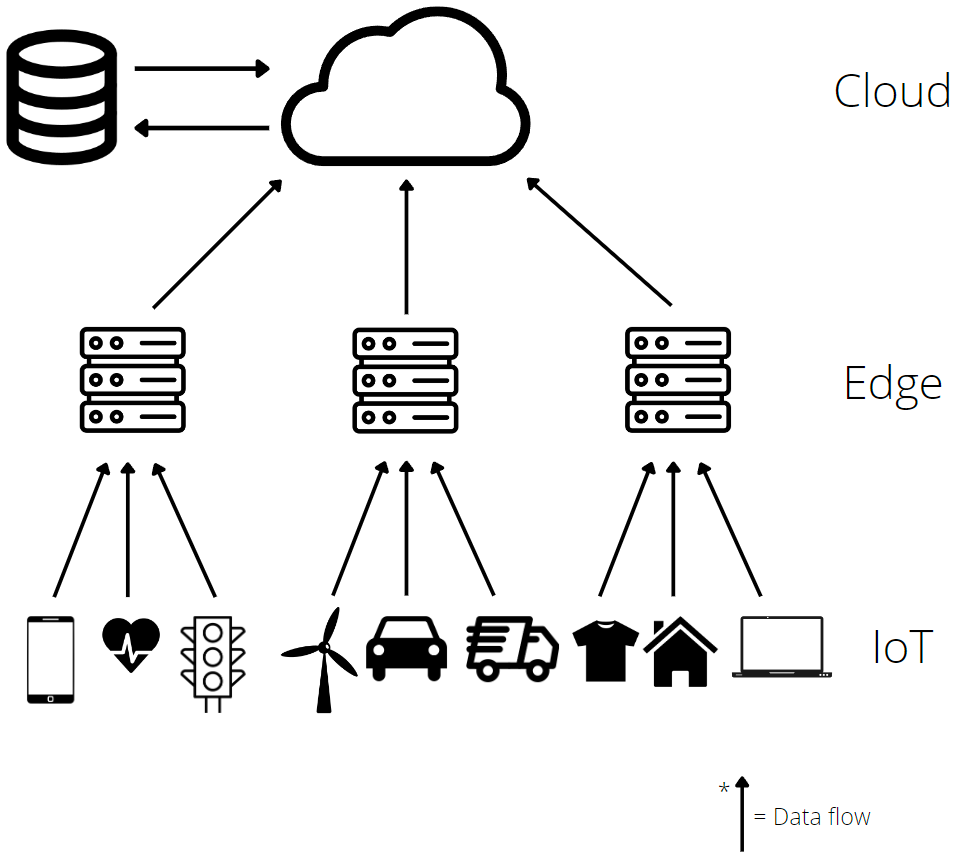
\includegraphics[scale=0.55]{images/cloud_edge_iot_stack.png}}
    \caption{Example of cloud-edge-IoT stack architecture}
    \label{fig:ceiot_stack}
\end{figure}

\subsection{Edge and Cloud Relationship}
Edge computing is considered an extension of Cloud computing and not a standalone computing paradigm; it still relies on the Cloud at the top level of its scheme, but it drastically reduces the load over the Cloud infrastructures while maintaining all of the Cloud's provided services like data computing, storage and applications. The main difference between the two is the location of the servers; with the Cloud alone, latency dependant applications may encounter latency and jitter issues due to the distance between the user device and the server. On the other hand, Edge computing enables location-aware and mobile applications with full support, while Cloud applications need to find other workarounds. The longer path to the server can also be a weak point for security attacks on the Cloud. Another difference is the target audience: Cloud computing is a global solution, Edge computing is limited. Lastly, the single Edge node hardware is designed to be horizontally scalable through distribution, while Cloud computing is generally more vertically scalable \cite{khan2019edge}.


Today, an ever-rising number of applications must use software that satisfies strict reliability, availability and integrity requirements, especially when dealing with critical safety systems; hence, multiple assurance and verification techniques have been introduced, such as certification schemes, testing, service level agreements, audit/compliance and monitoring frameworks \cite{ardagna2015security}. 


\section{Security and Assurance in Distributed Systems}
Software security assurance techniques enhance software and services transparency \cite{ardagna2014management} and increase the actors' confidence that such services behave as expected. In line with standard software security assurance definitions \cite{goertzel2007software}, cloud security assurance can be defined as the way to gain justifiable confidence that infrastructure and applications will consistently demonstrate one or more security properties and operationally behave as expected despite failures and attacks. However, assurance is a much wider notion than security, as it includes methodologies for collecting and validating evidence supporting security properties. When dealing with cloud infrastructure, Ardagna et al. \cite{article} highlighted three requirements that need to be considered with every assurance technique: i) risk assessment and management, ii) transparency and iii) public policy and compliance. 

Risk assessment and management are needed before the cloud service deployment and allow the business to obtain a precise evaluation of the risks that such a process would introduce. Transparency is a core component when defining and optimizing assurance techniques and allows end-users to visualize and control the data flow and the security issues in their services. In addition, transparency is necessary to support introspection, the capability of a cloud provider to examine and observe its internal processes, and outrospection, which is the same thing but from the customer's point of view \cite{ardagna2014management}. To comply with the transparency requirement, cloud providers must show their policies and compliance with standards and regulations and how such compliance is achieved \cite{macneil2006comply}. The major approaches to cloud assurance are discussed below.
\begin{description}
    \item[Testing]
    Testing involves executing software or system services with the help of manual or automated tools to evaluate specific behaviours and properties. The test activity allows gathering evidence to support the evaluation target's property; properties can belong to the cloud infrastructure or the service running on it.

    \item[Monitoring]
    Monitoring processes can be deployed to overcome the limits of direct testing approaches; it allows for gathering precise information about the status of services, events, and activities on the back end. In addition, the security of a cloud system can be greatly improved with monitoring approaches since they also increase transparency.

    \item[Certification]
    Various certification techniques have been developed to prove that a software system holds some non-functional properties and behaves as expected. The advantage of such techniques is the presence of a certificate released at the end of a successful process; such a certificate can then be shown as undisputable proof.
    
    \item[Audit and Compliance]
    An essential aspect of security and assurance is the capability of observing the system's behaviour and evaluating its compliance with customer policies and law regulations. Audit solutions have been developed with this very goal; additionally, they increase the system's transparency making systems like the cloud more accountable in case of issues and failures.
    
    \item[Service-Level Agreement (SLA)]
    SLA-based techniques establish contracts between clients and service providers, regulate their interactions, and model their expectations in functional and non-functional agreements \cite{article}.

\end{description}






\subsection{Security Certifications}
Security certifications are granted by independent (from the system supplier and acquirer) third parties whose goal is to verify the system's quality completely and objectively. Certifications allow more confidence in the product over the competition and legislative compliance when talking about quality, functionality and security \cite{heck2010software}. The certification schemes' main focus is to prove that the selected software system or service would have some non-functional properties and behave as expected. 
Over the years, there have been proposed two main types of certification approaches: i) static, such as the ones proposed by \cite{anisetti2013test}\cite{CSATrustSTAR} ii) continuous and incremental, such as Common Criteria \cite{anisetti2017semi}\cite{infrastructure2002common}. 

A generic software certification process requires two types of input: i) The software artefact that needs to be certified and ii) one or more Conformance Properties of the artefact. The properties usually fall into one of the following categories:

\begin{itemize}
    \item Consistency
    \item Functional
    \item Behavioural
    \item Quality
    \item Compliance 
\end{itemize}

Although in the most recent years, the NIST proposed to definitely classify the systems' properties under just the Confidentiality, Integrity and Availability categories, more about this in the [properties] chapter. Moreover, the properties can be generic or dedicated to the specific artefact and need to be appropriate to the application's domain; this is established in a Conformance Analysis process \cite{anisetti2017semi}.


\subsection{Certification Schemes History}
It is quite difficult to retrace the full history of software security certification schemes due to the vastity of the software products' types and the fact that many countries started developing their certification schemes when such products needed some form of assurance. For these reasons, software products requiring security properties resulted in having a rather steep way toward international distribution. Therefore, the first approaches started dealing with the main pillars of certification schemes, such as properties, models and evidence collection (Fig. \ref{Fig:OldProcess}). Starting from the history of the most known scheme, the Common Criteria, the first attempts at defining a standard approach to such a complex task were made between 1983 and 1993 with the Information Technology Security Evaluation Criteria (ITSEC), the Canadian Trusted Computer Product Evaluation Criteria (CTCPEC) and the Trusted Computer System Evaluation Criteria (TCSEC).
\begin{figure}[htb]
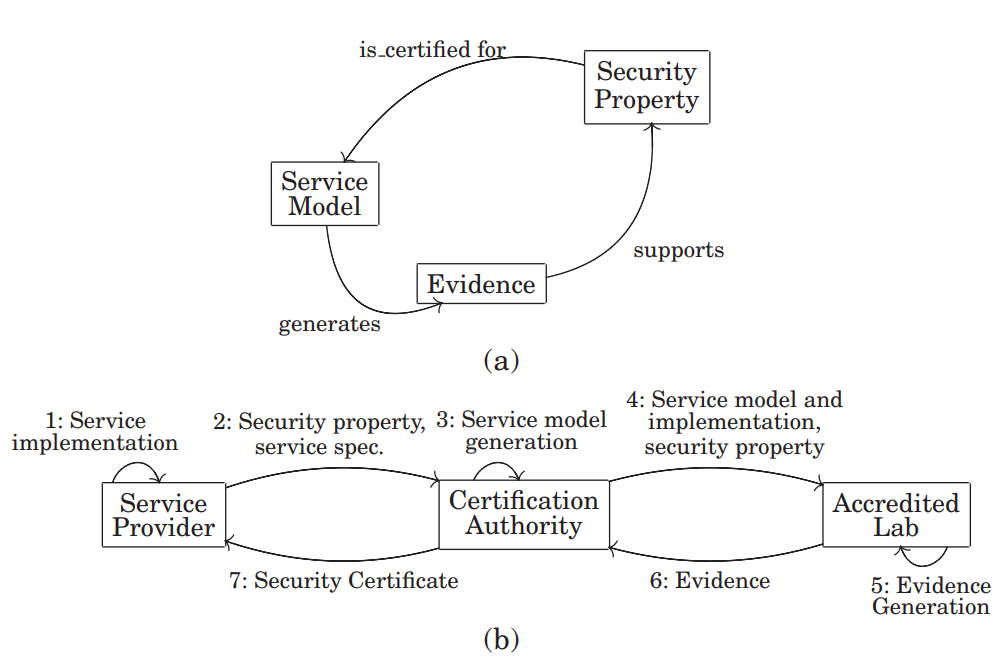
\includegraphics[width=\textwidth]{immagine_web_service.png}
\caption{Conceptual framework (a) and certification process steps (b) \cite{anisetti2013test}}
\label{Fig:OldProcess}
\end{figure}
\subsubsection{ITSEC}
ITSEC is a structured set of criteria with the scope of evaluating security within computer systems and products in the European Union; it was published in 1990 and was developed by France, Germany, Netherlands and UK governments, basing its features on the pre-existing, country-limited frameworks. This set of criteria was designed in the main part to be equally applicable to technical security measures in hardware, software and firmware products \cite{ITSEC}. ITSEC was centred around the Target of Evaluation (ToE) and assurance levels; these concepts made their way through all the versions of today's Common Criteria \cite{infrastructure2002common}.

\subsubsection{TCSEC}
TCSEC, commonly referred to as "The Orange Book" \cite{orangeBook}\cite{orangeBookDeath}, is a standard developed by the United States Government Department of Defense, and its scope was to evaluate and classify computer systems used for processing, storing and retrieving sensitive or classified information. This framework, like many others \cite{infrastructure2002common}\cite{ITSEC}, was developed around the following Evaluation Classes: 
\begin{itemize}
    \item D: Minimal Protection
    \item C1: Discretionary Security Protection
    \item C2: Controlled Access Protection
    \item B1: Labeled Security Protection
    \item B2: Structured Protection
    \item B3: Security Domains
    \item A1: Verified Design
    \item A2: Verified Implementation
\end{itemize}

\subsubsection{CTCPEC}
CTCPEC is a standard developed by the Canadian government with the same goals as ITSEC and TCSEC; in fact, it was a combination of the two. This approach finally led to combining the major standards and criteria into a single set: the Common Criteria \cite{CTCPEC}.

\subsubsection{Common Criteria}
\label{CC}
With these internationally approved standards, software companies finally had the tools to certify their products and sell them worldwide; however, every certification process had to be passed, resulting in a rather tedious and pricey process. Therefore, the Common Criteria (CC) was developed by unifying these pre-existing standards, following the approach of the CTCPEC, to allow companies to evaluate their products against a single set of standards. CC was developed by Canada, France, Germany, Netherlands, UK and USA governments and version 1.0 was issued in 1994; multiple agreements were signed in the following years to avoid useless re-evaluations and allow mutual recognition of CC certificates.
The Common Criteria for Information Technology Security Evaluation (also known as Common Criteria) represents the evolution of continuous and incremental certification schemes, and its latest versions are currently used to evaluate over two thousand major IT systems and applications (e.g. Microsoft Windows OS, McAfee anti-virus, Microsoft SQL Server \cite{CCProducts}).
CC is mainly based on the previous sets of standards' ideas:
\begin{itemize}
    \item Definition of the ToE, which includes the assignment of a Protection Profile, the description of the Security Target and the listing of the Security Functional Requirements.
    \item Definition of the Security Assurance Requirements
    \item Selection of the correct Evaluation Assurance Level
\end{itemize}

More details about the above phases are well described in \cite{infrastructure2002common}.

CC is now an established pillar in the security certification world, especially in the commercial industry, but it is not a perfect solution, especially when applied to highly dynamic systems like Edge and IoT. It is also worth noting that CC certifications are attributed to a specific version of the system under a specific configuration, and any configuration change or software update could mandate a re-certification process. To counter the redundancy of such processes, the CC designers proposed the Assurance Continuity (CCAC) re-evaluation process[], but the need to repeat the certification process is a big limitation. Therefore, the research never stopped; when considering highly dynamic domains such as those implied by the Cloud and Fog computing paradigms, it is important to define new certification schemes that better align with the context. 

%%%%%%%%%%%%%% da decidere se lasciarlo qui %%%%%%%%%%%%%%%%%%%%%%%%%


\subsection{Building Blocks of the Certification Schemes}
Modern certification frameworks rely upon several components defining how the process is executed and how the results should look. Below is a detailed list of the major pillars of certification frameworks with their fundamental functionalities as underlined by Anisetti et al. \cite{anisetti2017semi}\cite{anisetti2022multi}.

\subsubsection{Non-Functional Properties}
For the certification process of a system, it is important to establish some requirements that can be functional or non-functional preemptively, usually this is done during an initial risk assessment process. As stated by Chen et al. \cite{chen2013verification}: "broadly, functional requirements define what a system is supposed to do, and non-functional requirements define how a system is supposed to be", meaning that non-functional requirements focus on the system itself instead of what the system produces in output; once a requirement is proven to be satisfied by the system, it becomes a non-functional property of the same, and it can be expressed as follows: ⟨name, {(attribute, value), (attribute, value)}⟩. A property is composed of pairs "attribute-value" where the attributes are essential sub-properties that define the strength of the property. In other words, non-functional properties describe the system's capabilities and are usually grouped under the categories defined by the CIA triad: i) Confidentiality, ii) Integrity and iii) Availability. The CIA triad is an organizational model designed to guide information storing policies; its three parts are cybersecurity's three most crucial components. These properties are considered abstract because they represent generic security requirements and provide no information on how to achieve them. Instead, they are used to define concrete security properties. 

As defined by Anisetti et al. \cite{anisetti2013test}, a concrete security property is formally defined as follows:
A concrete security property, denoted \(p\), is a pair \( ( \hat{p}, A) \), where \(\hat{p}\) is an abstract property and \(A\) is a set of class attributes specifying the threats the service proves to counteract or the specific characteristics of the security function implemented by the service. 

The NIST defined these components as follows \cite{pub2005minimum}:
\begin{description}
    \item[Confidentiality] Preserving authorized restrictions on information access and disclosure, including means for protecting personal privacy and proprietary information. Confidentiality is a set of rules that limits access to information; ensuring confidentiality means the authorized entities can access the protected information and the unauthorized entities cannot. Confidentiality is accomplished through methods like data encryption and authentication procedures.
    \item[Integrity] Guarding against improper information modification or destruction, and includes ensuring information non-repudiation and authenticity. Integrity is the assurance that the information is trustworthy and accurate; it involves maintaining data consistency and accuracy over its entire lifecycle. For example, measures like file permissions and user access control ensure unauthorized entities cannot change data, while checksums and backups safeguard data from non-human threats like electromagnetic pulses or server crashes.
    \item[Availability] Ensuring timely and reliable access to and use of information. Availability guarantees reliable access to the information; it is best ensured by rigorously maintaining all hardware and staying up to date with all system upgrades; providing bandwidth, preventing bottlenecks and fast disaster recovery are also essential.

\end{description}



\subsubsection{Non-Functional Mechanisms}
For a non-functional property to be proven, a non-functional mechanism, in the form of \( ( name, \{ attribute, value \} )\), must be implemented to execute the certification process under specific configurations. Moreover, the property is what the process needs to verify, and the mechanism is the tool the system offers to test such property \cite{anisetti2017semi}; the verification is usually done through tests in the form of \\ \( (mechanism, (codde to execute, expected results))\). Finally, it is important to note that the mechanisms need to be described in the system's documentation; this allows the accredited laboratory to analyze and test them during the manual review phases.


\subsubsection{Target of Certification}
The application context and the system perimeter define the Target of the Certification (ToC); it describes the mechanisms on which the non-functional properties that need to be certified rely. Moreover, the evaluation of the certification scheme must verify the target’s (security) features. For example, in the Common Criteria process, the ToC (actually named Target of Evaluation) is accurately described in the Security Target Document.

\subsubsection{Evidence}
Evidence collection is the main step to proving that a given non-functional property is valid for a given ToC; it is important to note that evidence can be gathered by testing the service actively or passively. 
The property is finally assigned to the system when enough evidence is collected for a given requirement through well-aimed tests. 


\subsubsection{Life Cycle}
\begin{figure}[hb]
    \centering
    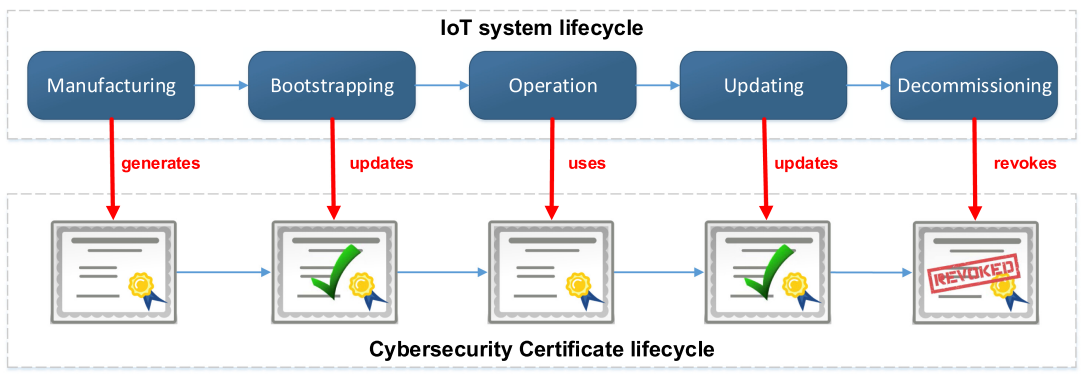
\includegraphics[scale=0.5]{images/lifeCycle.png}
    \caption{The cybersecurity certificate during the IoT device lifecycle.}
    \label{fig:lifecycle}
\end{figure}
As mentioned above, certificates are subject to invalidation, whether caused by a context change, a property change, or simply by the certificate's expiration; all certificates have a finite lifespan managed by the Certificate Authority (CA), which is usually also in charge of replacing it with a new one. However, the CA represents a bottleneck, and automation frameworks are needed when dealing with highly dynamic environments like Cloud and Edge. Therefore, the life cycle of a certificate is de facto a deterministic finite-state automaton whose state transitions are determined by specified conditions.

As mentioned above, certificates are subject to invalidation, whether caused by a context change, a property change, or simply by the certificate's expiration; all certificates have a finite lifespan managed by the Certificate Authority (CA), which is usually also in charge of replacing it with a new one. However, the CA represents a bottleneck, and automation frameworks are needed when dealing with highly dynamic environments like Cloud and Edge. Therefore, the life cycle of a certificate is de facto a deterministic finite-state automaton whose state transitions are determined by specified conditions. As shown in figure \ref{fig:lifecycle}, the lifecycle of a certificate is tightly coupled with the lifecycle of the IoT system, which is usually divided into five phases: i) Manufacturing, ii) Bootstrapping, iii) Operation, iv) Updating and v) Decommissioning. 

The manufacturing phase includes the production, programming and configuration of the system/device. This phase also includes the security certification process, which, if passed, assigns a brand new certificate to the system. The bootstrapping phase includes the installation and configuration of the device for the specific domain in which it will operate. Moreover, context-specific information should be embedded in the cybersecurity label (this step is too often ignored). It is also important to note that the context plays a fundamental role in every IoT system; a given device could require different security levels based on the type of information it needs to handle, and this variation can happen multiple times in the lifespan of the device. During the operation phase, the device/system provides its intended functionalities and should always be kept under a monitoring process. The monitoring is crucial to find new vulnerabilities and issues in the system. When a new vulnerability is found, and the manufacturer issues an update, rarely is a re-certification not issued due to the complexity of the analysis of the changes. Moreover, the security level and label are updated during a re-certification process. The decommissioning phase represents the end of the lifecycle of the system and includes the certificate revocation. This phase is also crucial because the devices composing the system could have stored sensitive information, and this phase's sole purpose is to make such information inaccessible \cite{surveyIOT}.

Typically, a certification process for Cloud services consists of a collaborative effort between four entities: i) a service provider who develops the service that needs to be certified, ii) a cloud provider supporting the service's certification, iii) a CA responsible for the definition of the requirements and the methodology and iv) an accredited lab to carry out the system evaluation. The problem of such an approach resides in the fact that continuous context changes can rapidly invalidate the assigned certificates, and without proper context testing techniques, it is necessary to re-certificate the whole service every time. The framework that M. Anisetti et al. proposed addressed this issue by constantly verifying the possessed certifications against the context changes to prevent unnecessary revocations and re-certifications.


\subsubsection{Labels}
Labelling schemes exist to straightforwardly inform the user about the security certification that has been executed on a device; such schemes should contain the following main groups of information:

\begin{itemize}
    \item Domain that was considered while performing the certification activity; the certification should be revoked the moment the device leaves it

    \item Level of assurance; states the security tests performed to certify the device. Usually, the level of assurance is associated with the protection profile of the specific domain

    \item  Information about the achievement of the certification, such as the responsible entity, the process and the validity period

\end{itemize}

Even though the importance of labels is mostly tied to commercial purposes \cite{baldini2016security}, perhaps, they could also be read by the Certification Authorities to have a quicker overview of the system's mechanisms and capabilities. In state-of-the-art schemes, labels are ignored or poorly used, but they might play a fundamental role in future schemes.


\subsection{Assurance for Highly Distributed Paradigms}
As described in section \ref{Edge}, Edge computing adds multiple challenges to the table in terms of functionalities, especially when combined with IoT layers, which bring on even more security and assurance topics. Mahmud et al. \cite{mahmud2018fog} highlighted three security aspects that will inherently haunt new highly distributed computing paradigms:
\begin{itemize}

\item Technological discoveries advance at different paces for software and hardware; new software architectures (like edge computing) are designed upon traditional components, especially for networking, raising the number of vulnerabilities to attacks.

\item Highly distributed systems make it difficult to ensure secure authentication and privacy in every node at all times; monitoring frameworks could be insufficient in many cases.

\item Security mechanisms for data-centric integrity can greatly affect the quality of service of these systems.

\end{itemize}



%%%%%%%%%%%%%%%%%%%%%%%%%%%%%%%%%%%%%%%%%%%%%%%%%%%%%%%%%%%%%%%%%%%%%

\subsection{New Certification Efforts in Cloud Environments}
Cloud service certification has been a highly focused research point in recent years and is now considered a mature assurance feature. Moreover, as identified by M. Anisetti et al. in \cite{anisetti2017semi}: "Compared to traditional service certification, cloud certification is: i) highly dynamic, it is affected by contextual changes at any layer of the cloud stack, ii) multi-layer, it can refer to services at different cloud layers; iii) intrinsically incremental, it requires continuous validity verification and incremental adaptation with the scope to minimize costly re-certification activities, and iv) trustworthy by delegation, it requires advanced trust models based on delegation to support cloud peculiarities". M. Anisetti et al. also proposed a continuous and incremental approach to Cloud service certification, providing a formal description of the audit-related evidence collection. Such an approach is founded on five main pillars: non-functional properties, non-functional mechanisms, Target of Certification (ToC), evidence collection and the life cycle of the certification. The proposed certification process can be simplified with the following steps: i) Non-functional properties definition, ii) ToC definition, which includes the description of the non-functional mechanisms offered by the system, iii) Tests definition, iv) Tests execution, which involves evidence collection and analysis and v) Certificate release.


This process involves different entities, such as the service provider, the cloud provider, the certification authority and an accredited laboratory; this way, a chain of trust is formed, and the responsibilities are evenly spread between the entities involved. It is also split into an issuing phase, where the process is responsible for all the evaluation activities, and a post-issuing phase, which continuously verifies the certificate's validity against eventual context changes \cite{anisetti2017semi}.

\subsection{New Certification Efforts in Edge Environments}
Certification schemes over Fog/Edge computing nodes are a recent and less mature topic; when dealing with a network composed of countless devices (the Fog nodes), it is fundamental to have a completely automated framework capable of handling the whole certification process for each node. The scheme proposed by Aslam et al. in \cite{aslam2020fonac} addressed the matter with automated and continuous monitoring and auditing of the Fog nodes; nevertheless, this total automation relies entirely on the backend provided by the Cloud infrastructure that acts as an inner CA for its Fog layer, inheriting all its vulnerabilities. The differences between this approach and the ones proposed for the Cloud are the requirements for the certifications. Fog nodes have limited functionalities and need to be quickly admitted to the Fog layer; meanwhile, there is a need to execute much stronger certification activities on the Cloud stack.

\subsection{Current IoT Certification Efforts}
Internet of Things is not a new concept, and so is not the need for dedicated certification schemes; The rapid spread of systems relying on IoT highlighted many limitations of the most known certification schemes.

\subsubsection{Common Criteria}
As described in section \ref{CC}, CC is the most used on every type of system (Cloud, Edge, IoT) thanks to its Mutual Recognition Agreements (MRA) and to the depth the certification process can reach. However, the industry and the research community have underlined three major limitations that make it hardly applicable in the IoT world \cite{kaluvuri2014quantitative}\cite{keblawi2006applying}:
\begin{enumerate}
    \item It takes too much time and effort, resulting in a slowdown of the system and the risk of overwhelming the single devices with testing requests.
    \item Systems classified with high EALs are attributed to highly complex documentation, making the comparison with other certificates difficult, hence, not complying with the harmonization challenge (more about this in the commercial section).
    \item Managing changes is almost non-existent, even with the CCAC version, limiting the number of updates the manufacturer can issue and drastically reducing system operativity during re-certification.
\end{enumerate}


\subsubsection{ICSA Labs IoT Security Testing Framework}
A newer framework is the one proposed by the ICSA Labs company. The ICSA Labs IoT Security Testing Framework is focused on IoT systems, more specifically, on the security of the single devices participating in an IoT environment. The approach is based on a periodic assessment and update of the certification criteria, and it includes frequent iterative updates, addressing the dynamic environment challenges and the evolving cybersecurity threats inherent to the IoT paradigm. This process is more focused on the iterativity of the assessments and less on the depth of the certification, leaving aspects such as the labelling ignored \cite{ICSAFw}.

CC remains the most used and studied certification scheme, while others like Commercial Product Assurance, Cybersecurity Assurance Program and the Certification de Sécurité de Premier Niveau fall into a commercial and country-specific side.


\subsubsection{Industrial And Commercial Purpose Schemes}
From the commercial and industrial point of view, several challenges have been highlighted in the definition and deployment of an IoT security certification framework; some of these are not part of this thesis' focus but are still relevant for a complete overview of what a certification framework should guarantee at a certain point; furthermore, table \ref{Tab:comparison} shows a quick comparison of the approaches discussed below.
\begin{enumerate}
    \item Standardization: Since the IoT landscape is still fragmented in approaches and standards, it is crucial to start aligning the efforts for a more homogeneous perspective.


    \item Harmonization: while there is the need to align the standards, there is also the need to allow different ones to coexist and be mutually accepted.


    \item Time, complexity and cost: Manual processes, direct testing and complex documentation guidelines of currently available approaches are heavy on resources like time and money, and the need to minimize this weight is crucial for a for-profit company, especially with IoT systems that need frequent re-certifications.


    \item Dynamic environment: IoT systems are often deployed in dynamic environments whose conditions might affect the security level of a device. Moreover, a device should be able to receive an update and change its or the system's configuration without invalidating the certificate completely.


    \item Influence of the context: The context in which an IoT system is deployed is not ignorable; indeed, it determines many of the security features the system will require. Moreover, the context and the system's purpose should be linked to determine the sensitivity of the managed data.


    \item Transparency to the end-user: A company must help the clients understand the positive aspects of the system's certification, especially when different approaches are not directly comparable. For this purpose, it is becoming a common rule to attribute security labels to the certificated devices; such labels should clearly and concisely represent the value of the certification's level. Labels' goal is ultimately to allow users to easily compare different levels of frameworks without knowing the approaches' details.


    \item Support for the certificate lifecycle: cybersecurity certificates carry validity periods that regulate and confirm the authenticity of the involved entities. It is important to ensure that the certification is supported and updated during its lifecycle and that all the certificated properties remain valid during this period.

\end{enumerate}


It should be noted that apart from the AC version of Common Criteria, no other approach considers a lighter process for re-certification processes.

Some available frameworks are adopted more frequently than others; in the following section, the most known and used in the industry will be presented and compared to highlight the major weaknesses that should be considered when developing new certification schemes \cite{surveyIOT}.

\subsubsection{Commercial Product Assurance}
The Commercial Product Assurance (CPA) is a certification scheme developed by the UK Communications-Electronics Security Group (CESG) for national public purposes. CPA allows only security-related patches and updates, and thanks to its "lightweight" design, it drastically reduced the re-certification process length; however, it is not enough. The average re-certification still takes at least six months to complete, reducing the system operativity during this time.

\subsubsection{Cybersecurity Assurance Program}
Cybersecurity Assurance Program (CAP) is a certification methodology developed by the Underwriters Laboratories company (UL) that adheres to their proprietary UL 2900 standards. Unfortunately, being a private and for-profit organization drastically reduces the community's trust in its certificates since they are not provable by third-party experts and do not adhere to the standardization and harmonization challenges.

\subsubsection{Certification de Sécurité de Premier Niveau}
The National Cybersecurity Agency of France developed certification de Sécurité de Premier Niveau (CSPN) in 2008 to verify the products' compliance with their security specifications in a timely manner. Unfortunately, this certification framework is standardized in France but not officially recognized by any other country, making it useless for international products.

%%%%%%%%%%%%%%%%%%%%%%%%%%%%%%%%%%%%%%%%%%%%%%%%%%%%%%%%%%%%%%%%%%%%%%%%%%%%%%%%%%

    


\begin{table}[htb]
    \centering
    \begin{tabular}{ |p{3cm}|p{2.3cm}|p{2cm}|p{2cm}|p{2cm}|p{2cm}|  }
         \hline
         \textbf{Challenges}&\textbf{CC}&\textbf{CPA}&\textbf{CAP}&\textbf{CSPN}&\textbf{ICSA Labs}\\
         \hline
         \textbf{Certification time (months)}* & 4-9 EAL2, 6-12 EAL3, 9-24 EAL4.
         & 6-18 & 6+ & 1-2 & 1-2\\
         \hline
         \textbf{Documentation} & Higher the EAL more complex the documentation & Hard to compare & Hard to compare & Hard to compare & Hard to compare\\
         \hline
         \textbf{Changes management} & Certificate valid only for specific patch and configuration & Any change is manually reviewed and can invalidate the certificate & Any change is manually reviewed and can invalidate the certificate & security patches invalidate the certificate & Any change is manually reviewed and can invalidate the certificate\\
         \hline
         \textbf{Context consideration} & \cmark & \xmark & Partially & \cmark & \cmark \\
         \hline
         \textbf{Monitoring} & \cmark & \cmark & \cmark & \xmark & \cmark \\
         \hline
         \textbf{Validity period} & Variable & Variable & 1 Year & 8 Weeks & 1 Year \\
         \hline
         \textbf{Labels completeness} & Only EAL info & \xmark & \xmark & \xmark & \xmark \\
         \hline
         \textbf{Mutual Recognition Agreements (MRA)} & Accepted by numerous countries & UK only & Not standard & France only & Not standard \\
         \hline
         \textbf{Cost (\$)}* & 75-200k EAL2, 110-250k EAL3, 150-350k EAL4 & 1300 per work day & Not standard & 25-30k & Not standard \\
         \hline
         \hline
         \multicolumn{6}{| c |}{\em*GAO analysis of data provided by laboratories.}\\
         \hline
    \end{tabular}
    \caption{Commercial Purpose Schemes Comparison}
    \label{Tab:comparison}
\end{table}


%%%%%%%%%%%%%%%%%%%%%%%%%%%%%%%%%%%%%%%%%%%%%%%%%%%%%%%%%%%%%%%%%%%%%%%%%%%%%%%%%%






\section{Configuration Changes}
A configuration change refers to modifying a component subject to change control. For example, some configuration changes that might interest an IoT system are the relocation of an asset (e.g. device, edge node, cloud server) or the change of some security property's attribute values.
Fields and attributes designated for change control are referred to as configuration information. There exist three main types of configuration change control \cite{IBMConfChange}:
\begin{description}
    \item[Configuration Change Tracking] Changes are tracked in the component record and automatically applied to the target attributes. This type of control can be paired with the other ones.
    \item[Revision Tracking] Based on revision versions that are incremented every time an update occurs. The revision records are used to support the configuration change tracking, which has to be present. This approach can also be combined with the approval-based change control, but when it is not, it is possible to change the configuration element directly in the component record.
    \item[Approval-Based Change Control] Configuration information cannot be altered without engineering change approval when this control change approach is involved. The evaluation involves using change or revision records to plan, approve and execute configuration changes; the used record is considered the engineering change record during this phase and provides core information about the history of past changes. Given the need for a configuration record, this approach can be combined with any other one.
\end{description}

Configuration changes represent a critical point in the cybersecurity certification frameworks because a certificate cannot predict how a system will be affected after one. Moreover, even though most developers are focusing on creating software that should not need a system restart after an update, the results are weak, and the system downtime represents another critical aspect for IoT systems. It should also be noted that an IoT system update includes the transferral of updated data and programs to all the devices composing it, resulting in a rather long downtime, depending on the system's topology and resources. Furthermore, downtime represents an issue for certification frameworks, especially for this thesis' proposed solution, due to the inability to start an evaluation process on the system.
To address the downtime matter, M. Ciok et al. recently proposed a platform to help developers with the system's architecture \cite{mateusz2022flex}.




\section{Looking Forward}
Certification schemes went a long way and passed through many iterations of improvements, optimizations and agreements; now, it is clear that no approach is perfect, especially when dealing with new generation systems that often include IoT layers in their stack. In addition, the IoT paradigm is much more dynamic than the cloud, both in the software and hardware, resulting in remarkably higher costs in terms of time and money; for this reason, the classic approaches seem not to be feasible anymore and result in being too restrictive for the IoT system manufacturers. The ideal certification scheme should be less rigorous in terms of assumptions and remove most costs (the manual phases). Such a scheme should deal with more variables, like unknown mechanisms, properties and attributes; a quick, ephemeral certification scheme that would verify only the strictly needed properties with the minimum effort to allow the system to keep operating right after remote configuration or context changes. Such an ideal scheme should address the following challenges:
\begin{enumerate}
    \item How should the properties be modelled now?\\ 
    As discussed in this chapter, current schemes rely on properties that are not expected to change, and their changes can lead to expensive, slow and redundant recertifications; finding new models for the system's properties is essential to allow manufacturers to keep updated their systems.
    
    \item Which of the other certification building blocks should change, and how?\\
    If the properties' model change, it is crucial to identify which of the other building blocks would be affected and which could be optimized.
    
    \item Remembering that some mechanisms might not be known, given a system and a property, what steps should be included in the new certification process to certify such property of the system?\\
    Non-functional mechanisms are usually known at certification time; this allows the laboratories to execute well-aimed tests to demonstrate the properties of the system exploiting such mechanisms. However, when dealing with dynamic systems, some configuration change could add or disable a mechanism which could not be easily detected; hence, it is important to design a scheme capable of dealing with this issue.
    
    \item How should the process deal with the limited resources of an IoT device/system in the testing phase?\\
    Downtime is another IoT system's major issue when dealing with recertifications. Some systems cannot afford to be disabled for long periods, but IoT devices have very limited resources. Minimizing the load and resorting to new testing methods could be needed to overcome this issue.
\end{enumerate}

The next chapter will focus on making the first step toward a new recertification scheme to address such challenges, specifically, challenges 1,2 and 4. It will introduce the scoring system and the trigger component that will make the process as fast and automated as possible; moreover, properties, attributes, evidence collection and certification will be remodelled and deeply discussed. Finally, the new models are introduced to obtain an extremely lightweight scheme that will allow manufacturers to recertify their systems with the minimum possible effort quickly.




\chapter{Methodology}
\label{cap3}

\chapter{Experiments}
\label{cap4}

\chapter{Conclusions}
\label{cap5}





%
%			BIBLIOGRAFIA
%
\begin{thebibliography}{00}

\bibitem{mell2011nist}Mell, P., Grance, T. \& Others The NIST definition of cloud computing. (Computer Security Division, Information Technology Laboratory, National …,2011)

\bibitem{atlam2017integration}Atlam, H., Alenezi, A., Alharthi, A., Walters, R. \& Wills, G. Integration of cloud computing with internet of things: challenges and open issues. {\em 2017 IEEE International Conference On Internet Of Things (iThings) And IEEE Green Computing And Communications (GreenCom) And IEEE Cyber, Physical And Social Computing (CPSCom) And IEEE Smart Data (SmartData)}. pp. 670-675 (2017)

\bibitem{khan2019edge}Khan, W., Ahmed, E., Hakak, S., Yaqoob, I. \& Ahmed, A. Edge computing: A survey. {\em Future Generation Computer Systems}. \textbf{97} pp. 219-235 (2019)

\bibitem{gokhale2018introduction}Gokhale, P., Bhat, O. \& Bhat, S. Introduction to IOT. {\em International Advanced Research Journal In Science, Engineering And Technology}. \textbf{5}, 41-44 (2018)

\bibitem{iorga2018fog}Iorga, M., Feldman, L., Barton, R., Martin, M., Goren, N., Mahmoudi, C. \& Others Fog computing conceptual model.  (2018)

\bibitem{sahni2018data}Sahni, Y., Cao, J. \& Yang, L. Data-aware task allocation for achieving low latency in collaborative edge computing. {\em IEEE Internet Of Things Journal}. \textbf{6}, 3512-3524 (2018)

\bibitem{yi2015fog}Yi, S., Hao, Z., Qin, Z. \& Li, Q. Fog computing: Platform and applications. {\em 2015 Third IEEE Workshop On Hot Topics In Web Systems And Technologies (HotWeb)}. pp. 73-78 (2015)

\bibitem{atlam2018fog}Atlam, H., Walters, R. \& Wills, G. Fog computing and the internet of things: A review. {\em Big Data And Cognitive Computing}. \textbf{2}, 10 (2018)

\bibitem{heck2010software}Heck, P., Klabbers, M. \& Eekelen, M. A software product certification model. {\em Software Quality Journal}. \textbf{18}, 37-55 (2010)

\bibitem{anisetti2017semi}Anisetti, M., Ardagna, C., Damiani, E. \& Gaudenzi, F. A semi-automatic and trustworthy scheme for continuous cloud service certification. {\em IEEE Transactions On Services Computing}. \textbf{13}, 30-43 (2017)

\bibitem{aslam2020fonac}Aslam, M., Mohsin, B., Nasir, A. \& Raza, S. FoNAC-an automated fog node audit and certification scheme. {\em Computers \& Security}. \textbf{93} pp. 101759 (2020)


\bibitem{baldini2016security}Baldini, G., Skarmeta, A., Fourneret, E., Neisse, R., Legeard, B. \& Le Gall, F. Security certification and labelling in Internet of Things. {\em 2016 IEEE 3rd World Forum On Internet Of Things (WF-IoT)}. pp. 627-632 (2016)

\bibitem{ardagna2015security}Ardagna, C., Asal, R., Damiani, E. \& Vu, Q. From security to assurance in the cloud: A survey. {\em ACM Computing Surveys (CSUR)}. \textbf{48}, 1-50 (2015)

\bibitem{infrastructure2002common}Infrastructure, P. \& Profile, T. Common criteria for information technology security evaluation. {\em National Security Agency}. (2002)

\bibitem{anisetti2013test}Anisetti, M., Ardagna, C., Damiani, E. \& Saonara, F. A test-based security certification scheme for web services. {\em ACM Transactions On The Web (TWEB)}. \textbf{7}, 1-41 (2013)

\bibitem{CSATrustSTAR}Cloud Security Alliance, Security CSATrust \& Assurance Registry (STAR). (\url{https://cloudsecurityalliance.org/star/}), Accessed: 2022-08-29

\bibitem{IBMConfChange}Configuration Change Overview. (\url{https://www.ibm.com/docs/en/mfnp/7.6.0?topic=changes-configuration-change-overview}), Accessed: 2022-08-29

\bibitem{mateusz2022flex}Mateusz Ciok, K., Pascual Espada, J. \& González Crespo, R. Flex-request: Library to make remote changes in the communication of IoT devices. {\em Expert Systems}. pp. e12994 (2022)

\bibitem{kaluvuri2014quantitative}Kaluvuri, S., Bezzi, M. \& Roudier, Y. A quantitative analysis of common criteria certification practice. {\em International Conference On Trust, Privacy And Security In Digital Business}. pp. 132-143 (2014)

\bibitem{keblawi2006applying}Keblawi, F. \& Sullivan, D. Applying the common criteria in systems engineering. {\em IEEE Security \& Privacy}. \textbf{4}, 50-55 (2006)

\bibitem{ICSAFw}Labs, I. ICSA Labs IoT Security Testing Framework. (\url{https://www.icsalabs.com/technology-program/iot-testing}), Accessed: 2022-08-29

\bibitem{surveyIOT}Matheu, S., Hernández-Ramos, J., Skarmeta, A. \& Baldini, G. A Survey of Cybersecurity Certification for the Internet of Things. {\em ACM Comput. Surv.}. \textbf{53} (2020,12), https://doi.org/10.1145/3410160

\bibitem{orangeBook}Latham, D. Department of defense trusted computer system evaluation criteria. {\em Department Of Defense}. \textbf{198} (1986)

\bibitem{ITSEC}Jahl, C. The information technology security evaluation criteria. {\em Proceedings-13th International Conference On Software Engineering}. pp. 306-307 (1991)

\bibitem{orangeBookDeath}Lipner, S. The birth and death of the orange book. {\em IEEE Annals Of The History Of Computing}. \textbf{37}, 19-31 (2015)

\bibitem{CTCPEC}Bacic, E. The Canadian trusted computer product evaluation criteria. {\em [1990] Proceedings Of The Sixth Annual Computer Security Applications Conference}. pp. 188-196 (1990)

\bibitem{CCProducts}Common Criteria Certified Products. (https://www.commoncriteriaportal.org/products/), Accessed: 2022-08-29

\bibitem{ardagna2014management}Ardagna, C., Asal, R., Damiani, E. \& Vu, Q. On the management of cloud non-functional properties: The cloud transparency toolkit. {\em 2014 6th International Conference On New Technologies, Mobility And Security (NTMS)}. pp. 1-4 (2014)

\bibitem{goertzel2007software}Goertzel, K., Winograd, T., McKinley, H., Oh, L., Colon, M., McGibbon, T., Fedchak, E. \& Vienneau, R. Software security assurance: a state-of-art report (sar). (INFORMATION ASSURANCE TECHNOLOGY ANALYSIS CENTER (IATAC) HERNDON VA,2007)

\bibitem{article}Ardagna, C., Asal, R., Damiani, E. \& Vu, Q. From Security to Assurance in the Cloud. {\em ACM Computing Surveys}. \textbf{48} pp. 1-50 (2015,7)

\bibitem{mahmud2018fog}Mahmud, R., Kotagiri, R. \& Buyya, R. Fog computing: A taxonomy, survey and future directions. {\em Internet Of Everything}. pp. 103-130 (2018)

\bibitem{macneil2006comply}MacNeil, I. \& Li, X. “Comply or Explain”: market discipline and non-compliance with the Combined Code. {\em Corporate Governance: An International Review}. \textbf{14}, 486-496 (2006)

\bibitem{anisetti2022multi}Anisetti, M., Ardagna, C. \& Bena, N. Multi-Dimensional Certification of Modern Distributed Systems. {\em IEEE Transactions On Services Computing}. (2022)

\bibitem{chen2013verification}Chen, M., Tan, T., Sun, J., Liu, Y., Pang, J. \& Li, X. Verification of functional and non-functional requirements of web service composition. {\em International Conference On Formal Engineering Methods}. pp. 313-328 (2013)

\bibitem{pub2005minimum}Pub, F. Minimum security requirements for federal information and information systems.  (2005)

\bibitem{nasiri2019security}Nasiri, S., Sadoughi, F., Tadayon, M. \& Dehnad, A. Security requirements of internet of things-based healthcare system: a survey study. {\em Acta Informatica Medica}. \textbf{27}, 253 (2019)

\bibitem{daemen1999aes}Daemen, J. \& Rijmen, V. AES proposal: Rijndael. (Gaithersburg, MD, USA,1999)

\bibitem{fischer2017dod}Fischer, T. DoD 5220.22-m data wipe method [US DOD wipe standard]. (Retrieved from Lifewire: https://www. lifewire. com/dod-5220-22-m-2625856,2017)

\bibitem{OpenSSLMan}Young, E. \& Hudson, T. OpenSSL Manual. , (\url{https://www.openssl.org/docs/man3.0/man7/crypto.html}), Accessed: 2022-09-13


\end{thebibliography}
% 
\end{document}


 
